Pour valider notre modèle, nous avons développé une simulation basée sur un graphe.
Chaque machine de notre système y est représentée par un nœud, et possède en moyenne \textit{l} liaisons vers d'autres machines (les liaisons sont fixées aléatoirement), comme présenté en \label{graph}.

\begin{figure}[ht]
\centering
     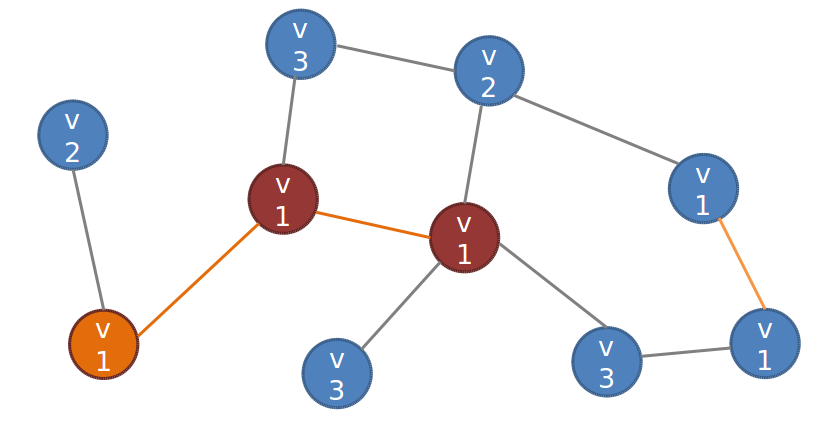
\includegraphics[width=1.0\linewidth]{Paul/python/graph.png}
     \caption{Représentation du système par un graphe}
     \label{graph}
\end{figure}

La première étape consiste à définir la répartition des logiciels dans le système. Afin de faire varier l'entropie, on utilise une distribution de Dirichlet. Celle-ci permet de s'approcher d'une distribution uniforme (proportions proches de $\frac{1}{n}$, grande entropie) ou au contraire de s'en éloigner (une proportion proche de 1 et les autres proches de 0, faible entropie). 

\begin{figure}[ht]
\centering
     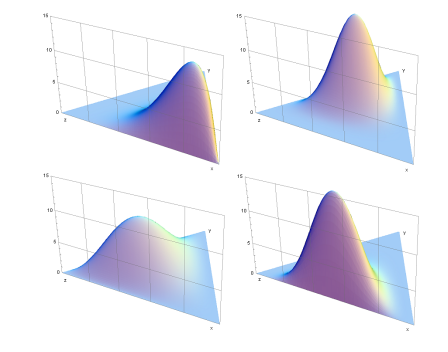
\includegraphics[width=1.0\linewidth]{Paul/python/dirichlet.png}
     \caption{Distribution de Dirichlet (source: Wikipedia)}
     \label{dirichlet}
\end{figure}

On répartit ensuite les logiciels au différents nœuds de manière aléatoires dans les proportions précédentes.
Pour chacun des logiciels du système, on prends aléatoirement l'un des nœuds sur lesquels il est présent comme le point d'entrée de l'infection. Les liens du graphe sont alors confirmés si chaque paire de nœuds correspondante est de cette version. Il ne reste alors qu'à compter le nombre de machines que l'on peut atteindre depuis la machine infectée initialement. Ce sera l'ensemble des machines infectées du système si l'attaque vise cette version.
On somme alors les cardinaux de tous ces ensembles, pondérés par la proportion de la version du logiciel correspondante dans le système.
On effectue cette simulation cent fois d'affilé pour chaque distribution, et la moyenne des résultats nous donne l'étendue moyenne de l'infection en nombre de machines infectées, pour l'entropie correspondante.


\begin{figure}[ht]
\centering
     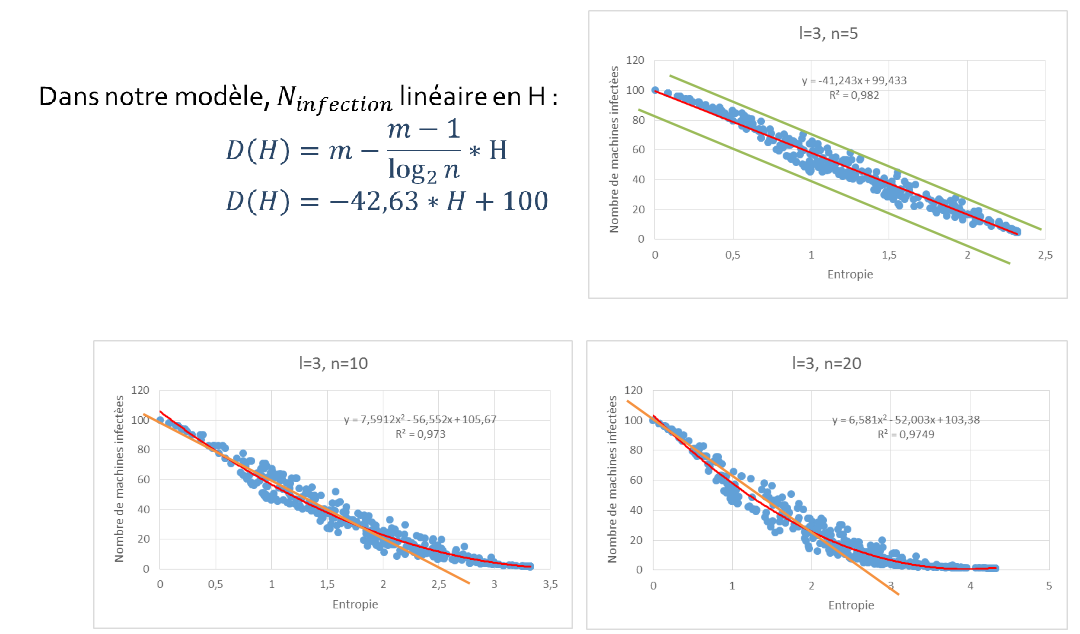
\includegraphics[width=1.0\linewidth]{Paul/python/lfixe.png}
     \caption{Simulation pour l fixé}
     \label{lfixe}
\end{figure}

\begin{figure}[ht]
\centering
     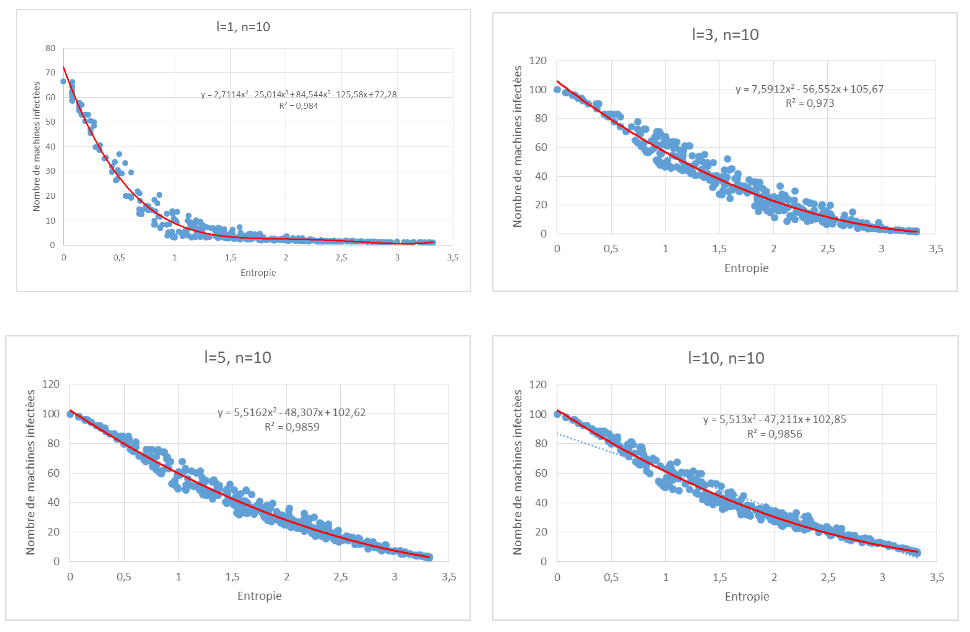
\includegraphics[width=1.0\linewidth]{Paul/python/nfixe.png}
     \caption{Simulation pour n fixé}
     \label{nfixe}
\end{figure}